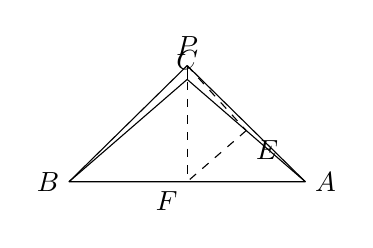
\begin{tikzpicture}[>=stealth, scale=1.5, line join=round]
  % 投影：x 向右，y 向屏幕内（0.5 压缩），z 向上（0.85 压缩）
  \coordinate (A) at (1,0);
  \coordinate (B) at (-1,0);
  \coordinate (C) at (0,0.866);
  \coordinate (F) at (0,0);
  \coordinate (E) at (0.5,0.433);
  \coordinate (P) at (0,0.983);
  % 棱
  \draw (A)--(B)--(C)--cycle;
  \draw (P)--(A);
  \draw (P)--(B);
  \draw (P)--(C);
  % 辅助线（中位线与等边三角形 PEF）
  \draw[dashed] (E)--(F);
  \draw[dashed] (P)--(F);
  \draw[dashed] (P)--(E);
  % 标注
  \node[right] at (A) {$A$};
  \node[left] at (B) {$B$};
  \node[above] at (C) {$C$};
  \node[above] at (P) {$P$};
  \node[below left] at (F) {$F$};
  \node[below right] at (E) {$E$};
\end{tikzpicture}
